\chapter*{Proposition 5}
\label{prop:5}

\begin{figure*}[ht]
    \begin{center}
    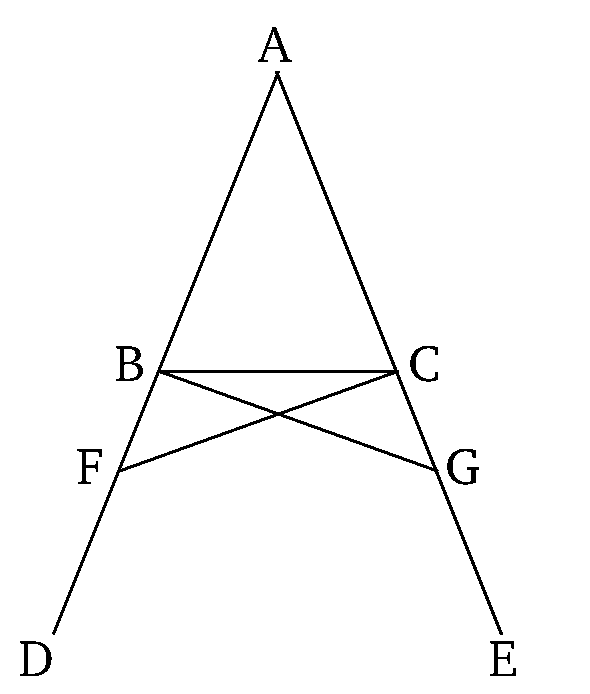
\includegraphics[width=0.5\linewidth]{figures/fig05e.eps}
    \label{fig:prop_5}
    \end{center}
\end{figure*}

For isosceles triangles, the angles at the base are equal to one another, and if
the equal sides are produced then the angles under the base will be equal to one another.

Let $ABC$ be an isosceles triangle having the side $AB$ equal to the side $AC$, and let the straight-lines $BD$ and $CE$ have been produced in a straight-line
with $AB$ and $AC$ (respectively) [Post.~\ref{post:2}]. I say that the angle $ABC$ is equal to $ACB$, and (angle) $CBD$  to $BCE$.

For let the point $F$ have been taken at random on  $BD$, and let $AG$
have been cut off from the greater $AE$, equal to the lesser $AF$ [Prop.~1.3]. Also, let
the straight-lines $FC$ and $GB$ have been joined [Post.~\ref{post:1}].

In fact, since $AF$ is equal to $AG$, and $AB$ to $AC$, the two (straight-lines) $FA$, $AC$ are
equal to the two (straight-lines) $GA$, $AB$, respectively. They also encompass a
common angle, $FAG$. Thus, the base $FC$ is equal to the base $GB$, and the
triangle $AFC$ will be equal to the triangle $AGB$, and the remaining angles
subtendend by the equal sides will
be equal to the corresponding  remaining angles [Prop.~1.4].  (That is) $ACF$ to $ABG$, and $AFC$ to $AGB$. And since the whole of $AF$ is
equal to the whole of $AG$, within which $AB$ is equal to $AC$, the remainder
$BF$ is thus equal to the remainder $CG$ [C.N.~\ref{cn:3}]. But $FC$ was also shown (to be) equal to $GB$. So
the two (straight-lines) $BF$, $FC$ are equal to the two (straight-lines) $CG$, $GB$, respectively,
and the angle $BFC$ (is) equal to the angle $CGB$, and the base $BC$ is common to
them. Thus, the triangle $BFC$ will be equal to the triangle $CGB$, and
the remaining angles subtended by the equal sides will be equal to the corresponding remaining angles [Prop.~1.4]. Thus, $FBC$ is equal to $GCB$, and $BCF$ to
$CBG$. Therefore, since the whole angle $ABG$ was shown (to be) equal to the
whole angle $ACF$, within which $CBG$ is equal to $BCF$, the remainder $ABC$
is thus equal to the remainder $ACB$ [C.N.~\ref{cn:3}]. And they are at the base of triangle
$ABC$. And $FBC$ was also shown (to be) equal to $GCB$. And they are under
the base.

Thus, for isosceles triangles, the angles at the base are equal to one another, and if
the equal sides are produced then the angles under the base will be equal to one another. (Which is) the very thing it was required to show.



\section*{Commentary}

\begin{proposition}\label{proposition_5}\lean{Elements.Book1.proposition_5}\leanok
    $|AB| = |AC|$ in $\triangle~ABC$. $AB$ is extended to $D$, and $AC$ is extended to $E$. Then, $\angle~ABC = \angle~ACB$ and $\angle~CBD = \angle~BCE$.
\end{proposition}
\begin{proof}
    \uses{proposition_3,proposition_4}\leanok
    See the original proof by Euclid.
\end{proof}

Euclid often use the following restricted version of Prop.~\ref{proposition_5} in later proofs.

\begin{proposition}\label{proposition_5'}\lean{Elements.Book1.proposition_5'}\leanok
    For $\triangle~ABC$, if $|AB| = |AC|$, then $\angle~ABC = \angle~ACB$.
\end{proposition}
\begin{proof}
    \uses{proposition_3,proposition_4,proposition_5}\leanok
    Extend $AB$ to $D$ and $AC$ to $E$. Then, $\angle~ABC = \angle~ACB$ by Prop.~\ref{proposition_5}.
\end{proof}